%!TEX TS-program = pdflatex
%!TEX encoding = UTF-8 Unicode
%!TEX root = ArsClassica.tex

\documentclass[a4paper,
		       titlepage,
               headinclude,
               footinclude,
               BCOR5mm,
               numbers=noenddot,
               cleardoublepage=empty,
               tablecaptionabove
               ]{scrreprt}

\usepackage[T1]{fontenc}

\usepackage[english,
            italian
            ]{babel}
            
\usepackage{amsmath,amssymb}

\usepackage{indentfirst}

\usepackage[style=philosophy-modern,
            hyperref]{biblatex}

\usepackage{chngpage}

\usepackage{calc}

\usepackage{listings}

\usepackage{graphicx}

\usepackage{subfig}

\usepackage{lipsum}

\usepackage{shapepar}

\usepackage{pifont}

\usepackage[eulerchapternumbers,subfig,beramono,eulermath,pdfspacing,listings]{classicthesis}

\usepackage{arsclassica}

% ********************************************************************
% Personal commands
% ******************************************************************** 
\newcommand{\myName}{Michele Papa}
\newcommand{\myTitle}{Vitres de Son}
\newcommand{\mySubTitle}{Come un rosone nel cuore di un tempio immenso}

\DeclareRobustCommand*{\clsname}[1]{{\normalfont\sffamily#1}}
\DeclareRobustCommand*{\pkgname}[1]{{\normalfont\sffamily#1}}
\DeclareRobustCommand*{\optname}[1]{{\normalfont\ttfamily#1}}
\DeclareRobustCommand*{\cmdname}[1]{\mbox{\lstinline[basicstyle=\normalsize\ttfamily]!\\#1!}}

\DeclareRobustCommand*{\classicthesis}{Classic\-Thesis}
\DeclareRobustCommand*{\arsclassica}{{\normalfont\sffamily ArsClassica}}


% ********************************************************************
% Hyper-references
% ******************************************************************** 
\newcommand{\mail}[1]{\href{mailto:#1}{\texttt{#1}}}


% ********************************************************************
% Graphics
% ********************************************************************
\graphicspath{{Graphics/}}


% ********************************************************************
% Code
% ********************************************************************
\definecolor{lightergray}{gray}{0.99}

\lstset{language=[LaTeX]Tex,
     keywordstyle=\color{RoyalBlue},
     basicstyle=\small\ttfamily,
     commentstyle=\color{Emerald}\ttfamily,
     stringstyle=\rmfamily,
     numberstyle=\scriptsize,
     showstringspaces=false,
     breaklines=true,
     frame=lines,
     backgroundcolor=\color{lightergray},
     flexiblecolumns=true,
     escapeinside={�*}{*�},
     firstnumber=last,
} 

\newcommand{\meta}[1]{$\langle${\normalfont\itshape#1}$\rangle$}

\lstset{	morekeywords=%
    {ProvidesPackage,RequirePackage,areaset,ifthenelse,%
     chapterNumber,undefined,boolean,DeclareRobustCommand,%
     spacedallcaps,textssc,MakeTextUppercase,lehead,%
     microtypesetup,textls,spacedlowsmallcaps,MakeTextLowercase,%
     sodef,allcapsspacing,lowsmallcapsspacing,thesection,%
     color,headmark,rohead,headfont,pnumfont,titleformat,%
     part,partname,thepart,chapter,thechapter,titlerule,%
     subsection,thesubsection,subsubsection,thesubsubsection,%
     paragraph,theparagraph,descriptionlabel,titlespacing,%
     formatchapter,textcolor,clearscrplain,rofoot,labelitemi,
     captionsetup,hypersetup}}

\lstnewenvironment{code}% 
   {\setkeys{lst}{columns=fullflexible,keepspaces=true}%
   \lstset{basicstyle=\small\ttfamily}}{}


% ********************************************************************
% Bibliography
% ******************************************************************** 
\bibliography{Bibliography}

\defbibheading{bibliography}{%
\cleardoublepage
\manualmark
\phantomsection
\addcontentsline{toc}{chapter}{\tocEntry{\bibname}}
\chapter*{\bibname\markboth{\spacedlowsmallcaps{\bibname}}
{\spacedlowsmallcaps{\bibname}}}}

\renewcommand*{\nameyeardelim}{\addcomma\space}

%-----------------------------------------------------------------------
%--------------------------------------------------- personalizzazioni -
%-----------------------------------------------------------------------

\usepackage{epigraph}

\usepackage{floatflt}

\usepackage{epsfig}

%-----------------------------------------------------------------------
%----------------------------------------------------------- documento -
%-----------------------------------------------------------------------

\begin{document}

\pagenumbering{roman}

\pagestyle{plain}

%!TEX TS-program = pdflatex
%!TEX encoding = UTF-8 Unicode

%*******************************************************
% Titlepage
%*******************************************************

\begin{titlepage}
\pdfbookmark{Titlepage}{Titlepage}
\changetext{}{}{}{((\paperwidth  - \textwidth) / 2) - \oddsidemargin - \hoffset - 1in}{}
    \begin{center}

\begin{table}[htp]
\begin{center}
\begin{tabular}{rl}
\multirow{ 2}{*}{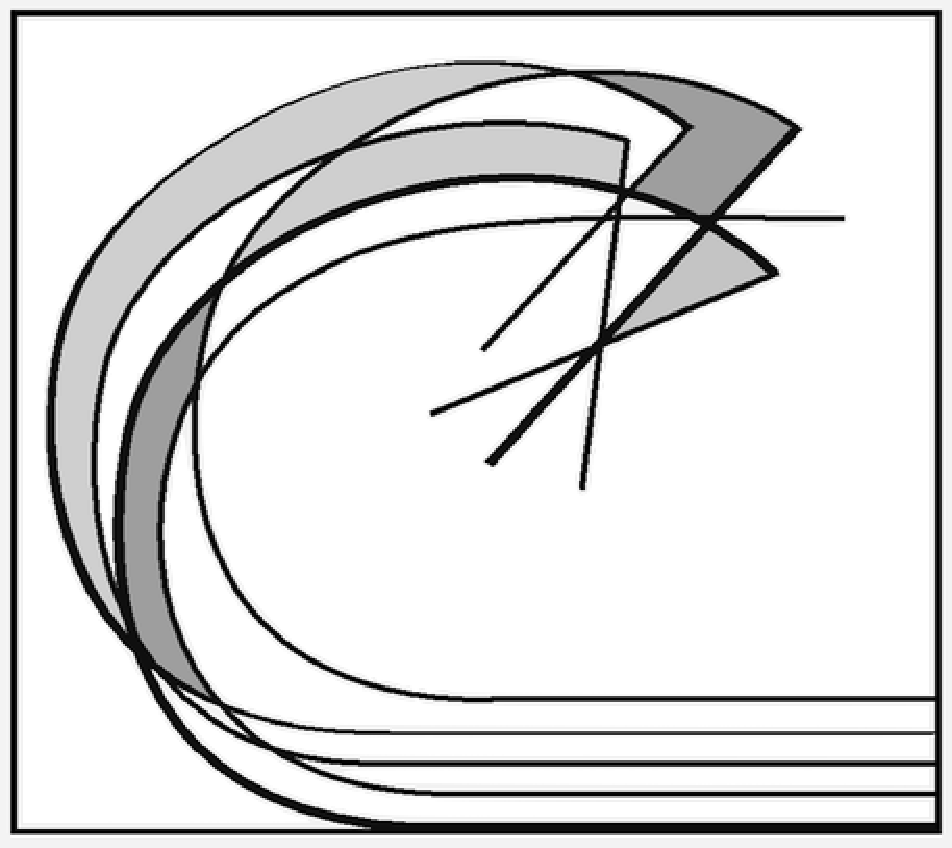
\includegraphics[scale=0.172]{Conservatorio.pdf}} & \LARGE \spacedlowsmallcaps{Conservatorio di Musica}\\ 
& \LARGE \spacedlowsmallcaps{S. Cecilia di Roma} \\ \cmidrule{2-2}
& \spacedlowsmallcaps{DIPARTIMENTO DI} \\
& \spacedlowsmallcaps{NUOVE TECNOLOGIE E LINGUAGGI MUSICALI} \\
& \spacedlowsmallcaps{SCUOLA DI MUSICA ELETTRONICA} \\
\end{tabular}
\end{center}
\label{default}
\end{table}%   

%        \LARGE \spacedlowsmallcaps{Conservatorio di Musica S. Cecilia di Roma}
%        
%        \bigskip
%        
%        \hrule
%        
%        \bigskip
%        
%        \large \spacedlowsmallcaps{DIPARTIMENTO DI NUOVE TECNOLOGIE E LINGUAGGI MUSICALI}
%        
%        \spacedlowsmallcaps{SCUOLA DI MUSICA ELETTRONICA}
        
		\vfill
        
        \spacedlowsmallcaps{CORSO DI DIPLOMA ACCADEMICO DI PRIMO LIVELLO IN}
                       
        \LARGE \spacedlowsmallcaps{MUSICA ELETTRONICA}

        \vfill ~ \vfill

        \LARGE {\color{Maroon}\spacedallcaps{\myTitle}}
        
        \large \mySubTitle 
        
        \vfill
        
        \normalsize Candidato: \\
        \Large \spacedlowsmallcaps{\myName}
        
        \normalsize Matricola: \\
        \Large \spacedlowsmallcaps{2945TR}
        
        \bigskip
        
        \normalsize Relatore: \\
        \Large \spacedlowsmallcaps{Michelangelo Lupone}

        \vfill ~ \vfill ~ \vfill
        
        \normalsize Anno Accademico: \\
        \Large \spacedlowsmallcaps{2016-2017}


%        
\includegraphics[width=0.7\textwidth]{TFZSuperEllisse} \\ \bigskip
                   

    \end{center}        

\end{titlepage} 

%!TEX TS-program = pdflatex
%!TEX encoding = UTF-8 Unicode
%!TEX root = ../2018-03-26-papa-vitres-de-son.tex

%*******************************************************
% Titleback
%*******************************************************
\thispagestyle{empty}
\pdfbookmark{Titleback}{Titleback}

\hfill

\vspace{\stretch{2}}

\begin{center}
Lorenzo Pantieri \\
\smallskip
\textit{The \arsclassica{} package}\\
\smallskip
Copyright\,\textcopyright\ 2008-2017
\end{center}
\vspace{\stretch{1}}

\medskip

\noindent\textsf{\spacedlowsmallcaps{Titleback}} \\
\noindent
This document was written with \LaTeX{} on Mac using \arsclassica, a reworking of the \classicthesis{} style designed by Andr\'e Miede, inspired to the masterpiece \emph{The Elements of Typographic Style} by Robert Bringhurst. 

\bigskip

\noindent
\textsf{\spacedlowsmallcaps{Contacts}}

\noindent
{\raisebox{-0.33ex}{\ding{43}}}\,\mail{lorenzo.pantieri@gmail.com}

\cleardoublepage

%!TEX TS-program = pdflatex
%!TEX encoding = UTF-8 Unicode
%!TEX root = ../2018-03-26-papa-vitres-de-son.tex

%*******************************************************
% Introduzione
%*******************************************************

\pdfbookmark{Introduzione}{Introduzione}

Ogni creazione artistica è legata imprescindibilmente sia alla carriera accademica che alla storia personale di chi la scrive. \\
Nel corso della stesura di questa tesi, ho cercato di esprimere il mio processo compositivo e creativo. La forma del testo, per una resa più diretta e scorrevole, è in forma romanzata, è una storia. Cercando in qualche modo di sfuggire da una semplice compilazione di liste sulle tecniche e sui materiali sonori utilizzati. \\
Questa composizione è più un sentiero da intraprendere ed è forse questo il lavoro che un compositore elettroacustico fa giornalmente: non la sola scrittura notazionale e simbolica, ma una continua ricerca di fenomeni che incarnino il proprio vissuto e nel quale un artista può identificarsi, facendoli suoi e riportandoli in musica, creando una propria identità artistica e formale. Come scrisse Kandisky nell'introduzione di \textit{Punto e linea nel piano}: 
\begin{small}
\begin{quotation}
\textit{Di ogni fenomeno si può fare esperienza in due modi. \\ Questi due modi non sono arbitrari ma connessi ai fenomeni -  essi vengono derivati dalla natura dei fenomeni, da due proprietà degli stessi: \\ 
\centerline{esterno - interno\footnote{Wassily Kandisky \textit{Punto e linea nel piano}, Adelphi Edizioni, Roma, 1968}.}}
\end{quotation}
\end{small}


Muovere \textit{interna}mente le corde della propria coscienza e delle proprie esperienze, provando a far vibrare ogni suggestione verso qualcosa di nuovo. Per "qualcosa di nuovo" non intendo un oggetto o una scrittura mai letta o vista prima. Il nuovo, penso, sia semplicemente l'unione di tecniche e di procedimenti fisici che per la prima volta subiscono quella successione di eventi nel tempo. Il tempo crea il nuovo nelle svariate possibilità che la vita ci propone: verso un \textit{esterno} dove abbiamo la possibilità di essere semplici ascoltatori o fautori dei cambiamenti che avvengono in tale realtà. 


\pagestyle{scrheadings}

% !TEX TS-program = pdflatex
% !TEX root = ../ArsClassica.tex

%*******************************************************
% Contents
%*******************************************************
\phantomsection
\pdfbookmark{\contentsname}{tableofcontents}
\setcounter{tocdepth}{2}
\tableofcontents
\markboth{\spacedlowsmallcaps{\contentsname}}{\spacedlowsmallcaps{\contentsname}} 

\cleardoublepage

\pagenumbering{arabic}

% !TEX TS-program = pdflatex
% !TEX root = ../ArsClassica.tex

%************************************************
\chapter{Sinossi}
\label{chp:Sinossi}
%************************************************

\textit{Vitres de Son - Come un rosone nel cuore di un tempio immenso} non � solo una composizione legata alla creazione e alla ricerca su un nuovo \textit{oggetto sonoro}, ma fa parte di un percorso compositivo e creativo che dura ormai da quattro anni. \\
Il titolo e il sottotitolo dell'opera sono rispettivamente il titolo e un verso di due poesie del drammaturgo, poeta e attore Antonin Artaud: \textit{Vitres de Son} e \textit{In Sogno}. Entrambe le poesie sono presenti in \textit{Poesie della crudelt�}\footnote{Antonin Artaud, \textit{Poesie della crudelt�} (a cura di P. Di Palmo), Stampa alternativa, Roma 2002, a cura di P. Di Palmo. Pubblicata per la prima volta nel 1925 \\}. \\
Artaud era artista ai margini, esponente del movimento surrealista e molto discusso dalla critica per le sue idee estremiste riguardanti il teatro, la messa in scena  e la modalit� di diffusione della sua arte:
\begin{small}
\begin{quotation}
\textit{Nell'epoca di confusione in cui viviamo, epoca colma di bestemmie e delle fosforescenze di un rinnegamento infinito, in cui tutti i valori sia artistici che morali sembrano sprofondare in un abisso senza altro esempio in nessun epoca dello spirito, ho avuto la debolezza di credere che avrei potuto fare un teatro, che avrei potuto almeno avviare il tentativo di ridare vita al valore universalmente disprezzato del teatro, ma la stupidit� di alcuni, la malafede e la spregevole canaglieria di altri me ne hanno distolto per sempre. } [...] \footnote{Antonin Artaud, \textit{Il teatro e il suo doppio}, Einaudi Autore, Roma 1968 \\}
\end{quotation}
\end{small}
L'artista spinge verso una critica sociale che lo porter� ai margini della societ� e nella quale mi rispecchio. Inoltre, la figura del drammaturgo si pu� accostare a quella dei \textit{clerici vagantes}\footnote{Furono cos� chiamati per tutto il sec. XII e il XIII quei poeti, che, vivendo al margine della chiesa, vagavano per le universit�, le citt� e le corti, spesso confusi con i giullari, di cui condividevano la vita errabonda e l'indole artistica. [...] \\ \textit{Enciclopedia Treccani} Edizione 2018. \\}. Sia Artaud che i clierici erano, infatti, personaggi solitari, irrequieti, artisti vaganti che risentirono quel potente risveglio intellettuale e politico della loro epoca (in entrambe le epoche), rispecchiandone le condizioni sociali ma soprattutto la fisionomia morale. L'artista � sempre stato un personaggio ai margini e soprattuto Artaud ha ricevuto non poche cure psichiatriche dopo essere arrivato a deliri tali da fermarlo anche nella sua produzione artistica. Per fortuna, le poesie utilizzate per la composizione del mio lavoro, sono legate al primo periodo artistico, quello giovanile, dove ancora riesce ad esprimere un proprio universo immaginifico. Il suo � un paesaggio fatto di personaggi e suoni, potrei azzardare quasi un \textit{paesaggio sonoro}, alla maniera di Schafer, dove ogni cosa, ogni suono, pu� diventare personaggio.
\begin{quotation}
[...] \\
come un rosone nel cuore di un tempio immenso. \\
E l� ascolteremo la cadenza immortale \\
delle linee e dei corpi ritmati \\
e di gotiche balaustre profumate \\
dalla dolcezza dei corpi amati \\
dagli uomini con grandi anime cadenzate, \\
\centerline{dai poeti profumati\footnote{Antonin Artaud, \textit{In Sogno} in Poesie della crudelt� \\}.}
\end{quotation}

Ecco, qui entra in gioco la fase di analisi e costruzione compositiva: l'unione di una visione - all'esterno - ascoltando, ad esempio, delle risonanze create da dita sui del rosone nel cuore del tempio immenso: riecheggiano - all'interno \footnote{qui faccio riferimento a \textit{Punto e linea nel piano} di Kandisky \\}- di un ambiente vuoto.
Al margine delle balaustre, assieme ad Artaud e i clerici vagantes, osserviamo i cambiamenti che avvengono sul linguaggio e sulla sua forma, sull'ambiente. \\
\begin{quotation}
\textbf{Vitres de Son} \\
Vitres de son o� virent les astres \\
verres o� cuisent les cerveaux \\
le ciel fourmillant d'impudeurs \\
d�vore la nudit� des astres. \\ \\ 
Un lait bizarre et v�h�ment \\
fourmille au fond du firmament \\
un escargot monte et d�range \\
la placidit� des nuages. \\ \\ 
D�lices et rages, le ciel entier \\
lance sur nous comme un nuage \\
un tourbillon d'ailes sauvages \\
torrentielles d'obsc�nit�s\footnote{Artaud, \textit{Vitres de Son} in Poesie della crudelt� \\}. \\
\end{quotation}
I \textit{Vetri di suono} diffondono un materiale acustico fascinoso sia nella forma di diffusione elettroacustica che nella tipologia del gesto: mentre l'eccitazione delle armoniche e la componente elettronica, ci spingono verso l'alto, la vibrazione delle sub-armoniche di grandi molle \footnote{vedi cap. 2 \\} ci terr� con i piedi ben saldi al pavimento antistante alla cattedrale, per me astrazione immaginifica della sala da concerto. \\
Davanti a questo universo fatto di paesaggi e personaggi sonori, entra in causa la composizione. Il processo compositivo legato alle immagini e al ritmo dei versi di Artaud sar� il fulcro dominante dell'andamento formale di \textit{Vitres de Son - Come un rosone nel cuore di un tempio immenso}.

% !TEX TS-program = pdflatex
% !TEX root = ../ArsClassica.tex

%************************************************
\chapter{L'opera Sp.I.R.E}
\label{chp:L'opera Sp.I.R.E}
%************************************************
\chapter*{2. L'opera SP.I.R.E.}
\addcontentsline{toc}{chapter}{2. L'opera SP.I.R.E.}

\epigraph{[...] bello come la retrattilit� degli artigli degli uccelli rapaci; o ancora, come l'incertezza dei movimenti muscolari nelle pieghe delle parti molli della regione cervicale posteriore; [...] e soprattutto, come l'incontro fortuito su un tavolo di dissezione di una macchina da cucire e di un ombrello!}{Isidore Lucien Ducasse \\}

Tutto ebbe inizio nel luglio del 2017. \\
Nel corso della manifestazione \textit{ArteScienza} al Goethe Institute venne invitato il compositore francese, Pierre Jodlowski. Il suo lavoro compositivo \textit{Ombra della Mente} � ispirato ad alcuni scritti di Alda Merini durante le sue ricerche nei reparti psichiatrici. \\
Il lavoro di Jodlowski era basato su una parte teatrale recitata e una parte suonata da una clarinettista e cantata da una soprano (la stessa performer della voce recitante). La fusione tra momenti prettamente teatrali e parti musicali ebbero un effetto tagliente sulla mia produzione musicale successiva. Ogni intervento recitante era contrappuntato da rumori di strofinio di una matita su un foglio di carta e la frizione di una piccola molla presente nella meccanica della lampada di scena posizionata su uno scrittoio in palcoscenico. Tutto elaborato in live electronics. L'effetto della molla sfregata, amplificata da un microfono a contatto, mi ha fatto riaffiorare alla mente molti concerti di musica underground seguiti in passato (l'utilizzo delle molle, oltre ad appartenere all'universo della musica colta � stato abusato in ambienti musicali \textit{noise}\footnote{genere che utilizza il rumore come base principale per creare delle composizioni} e di musica cosiddetta "industriale" proprio per sottolineare l'utilizzo di materiale di scarto di industrie e fabbriche).
\begin{quotation}
Il paesaggio sonoro \textit{lo-fi} nasce dalla congestione sonora\footnote{R. Murray Schafer, \textit{Il paesaggio sonoro}, Casa Ricordi s.r.l. e LIM edizioni, 1985 \\}.
\end{quotation}
Andando avanti negli studi ho notato, poi, che gi� negli anni 50 del Novecento, John Cage cerc�, tramite l'utilizzo di elettromagneti e microfoni, di far percepire, amplificandoli, dei suoni non udibili. Dopo aver percorso durante il corso di \textit{interpretazione del partitura elettroacustica} assieme al M� Giuseppe Silvi, tutto lo scenario cagiano, ho iniziato ad interessarmi in modo pi� serio all'universo delle molle e alle loro particolarit� timbriche. Durante le mie ricerche � stato fortuito il lavoro fatto assieme al maestro Michelangelo Lupone al Centro di Ricerche Musicali (CRM) sito in Roma. \\
Aiutai il maestro alla creazione di una sua installazione nell'estate del 2017 assieme all'artista Licia Galizia: la scenografia interattiva della spettacolo coreutico \textit{Corpus 2.0}. L'utilizzo dei diffusori che montavamo all'interno delle opere installative e l'utilizzo di trasduttori piezoelettrici come parametri di controllo, mi ha fatto avvicinare ad un mondo a me limitrofo ma in parte sconosciuto. \\

\section{Necessit� di uno strumento dedicato}
\addcontentsline{toc}{section}{Necessit� di uno strumento dedicato}

Durante le giornate di lavoro al CRM ogni materiale diventava fonte di ricerca sul suo utilizzo e sulle capacit� timbriche. Ogni oggetto sonoro diventava frutto di studi sul timbro, anche minimi a volte per via dei tempi brevi dati dalle consegne, ma pieni di un universo sonoro al quale aggrapparsi. \\
Giorno per giorno si andava a materializzare un'idea sempre pi� nitida, fino al giorno del mio esame del III anno di composizione elettroacustica. \\
Un esercizio, un brano, un piccolo studio sulle armoniche del pianoforte, dove tutto partiva dalla trasformazione di un gesto sonoro, il pedale di risonanza in \textit{\textbf{fff}} e da una cellula sonora dalla quale poi, si formavano e alternavano momenti inarmonici con cluster e piccole volatine. Gesti e cellule sonore venivano elaborate tramite tre convoluzioni. Ogni convoluzione apparteneva ad un universo sonoro a s�:
\begin{itemize}
\item{la prima convoluzione era la stessa cassa di risonanza del pianoforte eccitata dal pedale di risonanza calcato in \textit{\textbf{fff}};}
\item{la seconda convoluzione era creata registrando la molla della stessa lampada da tavolo utilizzata da Pierre Jodlowski nel suo lavoro;}
\item{la terza convoluzione era un'eccitazione del manico di una chitarra elettrica su un amplificatore a transistor.}
\end{itemize}

\begin{floatingfigure}{10cm}
\mbox{\epsfig{file=Prototipo0.jpg,width=9cm}}
\small{\caption{\textit{particolare}}}
\end{floatingfigure}
Ogni convoluzione era quindi legata ad un gesto. Da qui alla creazione del mio iper-strumento, il passo � breve. Riuscii finalmente ad avere del tempo per finire di progettare il basamento, che prontamente un mio collega, Leonardo Mammozzetti ha provveduto a costruire, cos� da poter finalmente vedere e soprattutto sentire se tutte le mie idee portavano a qualcosa di reale. Era nato lo Sp.I.R.E. \\

\textit{Sp.I.R.E.}, acronimo di \textit{Springs Installation Regulated \& Enhanced}, fa riferimento alla fisicit� del materiale che compone lo strumento. Ogni molla (\textit{spring}) � formata da \textit{spire}. Il numero di tali spire rende possibile, a seconda del materiale col quale vengono eccitate le molle, l'attivazione di armoniche e/o sub-armoniche. \\
\begin{floatingfigure}{10cm}
\mbox{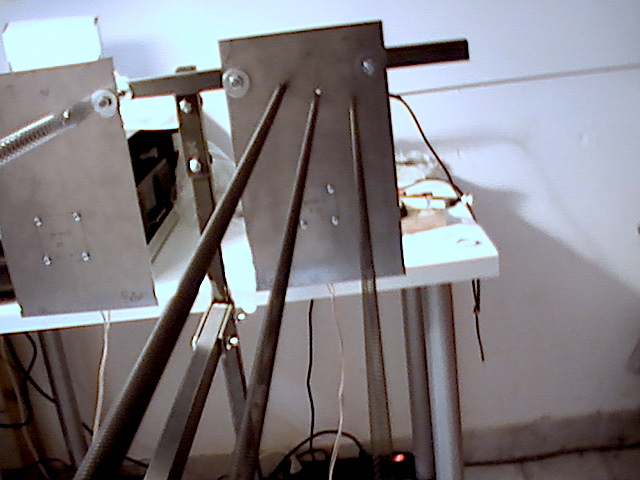
\epsfig{file=Prototipo2.jpg,width=8cm}}
\small{\caption{\textit{particolare}}}
\end{floatingfigure}
User� quindi l'appellativo di Iper-strumento, perch� � a tutti gli effetti uno strumento elettroacustico. \\
Questo esperimento � connesso allo studio di nuove identit� formali relative alla natura dello strumento musicale.  La ricerca � unita ad una realt� installativa dell'opera, che induce chi guarda e ascolta, a toccare la materia e ad incuriosirsi verso materiali come molle e placche di metallo, che sono stati creati per scopi lontani dall'utilizzo che ne viene fatto in questo determinato caso. \\
Spiego sinteticamente. Un basamento unisce due placche di metallo che montano su di esse, 3 molle ciascuna, tese per la lunghezza paritaria di 80 centimetri.\\
Sp.i.r.e. � un progetto ambizioso che vuole, tra le altre cose, reinterpretare ed ampliare la visione di John Cage in Cartridge Music. Riuscire a rendere percepibili i suoni non udibili,  impercettibili, prodotti da una serie di molle a trazione, opportunamente amplificate, presenti sulla struttura. \\
Le molle sono disposte sul materiale a gradini, come se si andasse a suonare un violoncello, o un contrabbasso in posizione orizzontale. 
Ogni movimento sar� legato alle immagini di cordofoni classici, quindi durante la performance l'esecuzione avverr� con l'utilizzo di archetti per violoncello e contrabbasso. Da qui l'evoluzione del materiale in percussione o semplicemente in risonatore. 
L'installazione sar� interattiva: ogni tocco ricevuto dalle molle modificher� il segnale di sintesi che verr� propagato tramite gli attuatori, fissati sulla parete metallica.


\section{Intenzioni espressive}
\addcontentsline{toc}{section}{Intenzioni espressive (ideazione)}
\epigraph{\textbf{spirare} v. intr. e tr. [lat. spirare �soffiare�; respirare; emanare�]"}
{\textit{Enciclopedia Treccani}}

L'intenzione espressiva era perci�, la creazione di uno strumento che avesse in s� sia un reverbero a molle che un reverbero a piastra. Il risultato fu esaltante: le molle sfregate con dita o archetti generavano un ambiente sonoro che le piastre amplificavano, dando vita a una sorta di convolutore naturale. So di estremizzare il senso di convoluzione, anche perch� come sappiamo il convolutore � una sommatoria tra due segnali, uno legato ad un ambiente di ripresa e uno legato ad uno strumento suonante. \\
\begin{floatingfigure}{10cm}
\mbox{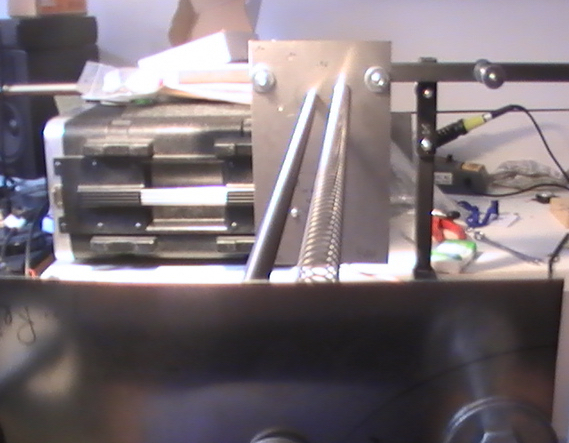
\epsfig{file=Prototipo3.jpg,width=9cm}}
\small{\caption{\textit{particolare}}}
\end{floatingfigure}
La svolta decisiva la ebbi durante il montaggio di Sp.I.R.E. perch� decisi di aggiungere una variante elettroacustica: aggiunsi degli attuatori. Gli attuatori, diffusori a parete capaci di far interagire il materiale sul quale sono collocati con il suono diffuso, erano la variante finale per la messa a punto finale dell'opera.
Come scrive Silvia Lanzalone:
\begin{quotation}
}La catena elettroacustica, nonostante il notevole perfezionamento tecnologico degli ultimi decenni verso l'accuratezza della riproduzione sonora, conferisce ancora al suono una trasformazione finale dovuta alla natura elettromeccanica dei suoi componenti, imponendovi dunque una deformazione che la rende decorrelata dal segnale che trasmette, nonch� estranea ad esso dal punto di vista della sua identificazione percettiva nello spazio destinato alla sua diffusione}\footnote{Silvia Lanzalone \textit{Strumenti aumentati} in \footnote{Acustica} UTET}.
\end{quotation} 

Spesso, quasi sempre, il suono elettronico risulta 

Per messa a punto finale intendo ovviamente la creazione di un ambiente di lavoro da quale partire per poter sia iniziare i primi studi sul timbri, ma soprattutto, per iniziare a scrivere una composizione scritta ad hoc per Sp.I.R.E.. \\

\section{Intenzioni estetiche}
\addcontentsline{toc}{section}{Intenzioni estetiche}
Il progetto va a rappresentare il legame con ci� che abbiamo attorno a noi, quello che siamo: tutt'uno con la metropoli e con l'ambiente che la circonda e va a formarla. \\
Questa � l'identit� di Sp.i.r.e., finalmente si tocca con mano la parte nascosta della materia, il lato pi� nascosto di quello che vediamo attorno a noi. In unione ai suoni non udibili e all'invisibile, si scorge un richiamo verso una visione immaginifica che porta fino a dentro la nostra anatomia. Come se le spire della molla potessero essere ricondotte ai ripiegamenti dell'intestino; come se, all'eccitazione di una molla, si riconducesse la possibilit� di produrre delle sub-armoniche e in qualche modo, di avvicinarsi alle vibrazioni interne dell'anatomia umana.\\
La meccanica, l'elettronica e i suoni analogici, rendono possibile la creazione di un mondo nuovo, e l'eccitazione delle molle mediante le placche di metallo fa s� che questa dimensione diventi parte della realt� umana. \\
Vengono a formarsi pi� dimensioni d'ascolto e pi� dimensioni tattili, causate dalle diverse eccitazioni del materiale. A queste dimensioni d'ascolto si unisce la diffusione audio della performance, che sar� omnidirezionale e render� possibile coprire tutto il panorama d'ascolto. \\
Cos� Sp.i.r.e., anche nella sua identit� installativa, respira ed emana il segnale elettroacustico in almeno due dimensioni d'ascolto:
\begin{enumerate} 
\item{\textit{Analogica}, la risposta del materiale ai suoni sintetici e al tocco umano}
\item{\textit{Elettrica ed elettronica}, che prende vita grazie ai suoni di sintesi diffusi dagli attuatori}
\end{enumerate}



% !TEX TS-program = pdflatex
% !TEX root = ../ArsClassica.tex

%************************************************
\chapter{La Performance}
\label{chp:La Performance}
%************************************************

Le difficolt� che intercorrono nel rapporto musicale con il performer sono legate anche al simbolo e alla consequenzialit� temporale della notazione. Mi riferisco in particolare al numero di gesti da eseguire sulle molle o sulle placche e alla mancanza di una notazione standard che pu� far perdere la consequenzialit� di tali gesti. \\
Simboli e ritmica, quindi, devono essere puntuali soprattutto nelle parti in cui due gesti o due figure si incastrano tra di loro. Sicuramente, la notazione metronomica e l'utilizzo di accenti � essenziale per la buona riuscita del pezzo, perch�, in qualunque caso, si vanno a delineare le micro-forme e la struttura principale del pezzo.

\section{Legame tra esecutore/performer e compositore}
\addcontentsline{toc}{section}{Legame tra esecutore/performer e compositore}


\epigraph{I TEMI \\ Non si tratta di opprimere il pubblico con preoccupazioni cosmiche trascendenti. Che possano esservi chiavi profonde del pensiero e dell'azione in base alle quali leggere tutto lo spettacolo[...]. Tuttavia � necessario che queste chiavi esistano; e la cosa riguarda noi.}{\textit{Antonin Artaud \\ Il teatro e il suo doppio}}

Nel lavoro intercorso con l'esecutore, Matteo Fracassi, studente del dipartimento di Percussioni del Conservatorio Santa Cecilia, ho riscontrato delle difficolt� nel far recepire il contenuto timbrico e dinamico dei gesti. Il legame tra gesto e figura � strettamente correlato, dato che, l'approccio ad uno strumento nuovo ha bisogno di uno studio puntuale sull'utilizzo delle dinamiche e sul capire la correlazione tra il gesto scritto e risultato sonoro. Ogni gesto avr� bisogno di un riscontro sonoro adeguato per evitare che la timbrica stessa di questo nuovo strumento porti a rapportarcisi in modo pi� improvvisativo che di studio, dalla la natura accattivante del suono in uscita da Sp.I.R.E.. In pratica, ogni gesto rappresentato in partitura sar� la risultante sonora di un determinato timbro o di una determinata ricerca di armoniche possibile sullo strumento. Il performer diventa quindi un essere mitologico, a forma di esecutore, ma con una capacit� performativa estesa alla conformazione dello strumento. Una figura complessa che deve avere la capacit� di seguire una struttura compositiva che cercher� di essere la pi� salda possibile e oltremodo precisa. Questo � la parte da esecutore. Quindi, riuscire districarsi nella lettura di una scrittura "quasi" libera. Per quasi, si intende la libert� minima a livello temporale di prendersi le giuste pause, ma allo stesso tempo riuscire a legare i vari fraseggi che si incastrano, restringono, dilatano nel tempo (durata delle frasi) e nello spazio (estensione dello strumento).


% !TEX TS-program = pdflatex
% !TEX root = ../ArsClassica.tex

%************************************************
\chapter{La Composizione}
\label{chp:La Composizione}
%************************************************

Durante questi anni di accademia ho trasformato il mio rapporto con la composizione e il metodo di approccio agli strumenti e alle forme musicali. Dapprima ero in balia di un lungo
Il mio approccio alla composizione 
Come ogni mio attuale approccio a livello compositivo, ho cercato di creare una cellula di suoni disposti orizzontalmente, per poi lavorare sulla parte contrappuntistica. Dato che il nuovo strumento non ha pitch definiti � stato complicato lavorare su una cellula che al finire del suo svolgersi si potesse definire conclusa. Difatti ho cercato degli stratagemmi musicali, come gli accenti o la ricerca di determinati effetti timbrici (ad esempio attivazione di armoniche sugli estremi delle molle) che potessero diventare dei gesti musicali, sia a livello grafico che a livello d'ascolto. L'insieme di accento o di un numero determinato di gesti, vanno a formare le mie cellule ritmico-melodiche che interagiscono con la materia di cui � composta Sp.I.R.E. e quindi sempre in un rapporto 1:1 tra il ferro armonico delle placche e il metallo armoniche delle molle. Ogni cellula si sovrappone poi ad altre cellule simile in piccoli inserti contrappuntistici fatti di dilatazioni o restrizioni temporali del materiale sonoro. \\ 
Le cellule ritmiche sono formate da 7, 6, 5 e 11 eventi. La numerologia � legata al numero delle lettere che compongono nome e cognome dell'autore della poesia (7 = A-n-t-o-n-i-n, 6 = A-r-t-a-u-d), al numero delle sillabe del suddetto nome+cognome (5) e dal numero dei versi della poesia (11) sopra citata. \\
A livello compositivo compaiono delle cellule ritmiche che vanno a confluire in grossi nubi sonore. L'attinenza tra la scrittura e il gesto a volte � slegata, ma le piccole note e la tendenza ad una continuit� ?notazionale? porta l?esecutore-performer a capire in quali punti vanno gestiti dei continuum. \\
Su ogni continuum vanno a frammentarsi altre cellule ritmiche. Ogni cellula si ripete, ma con piccole variazioni temporali, ogni gesto � riconosciuto sia nella semiografia che dal timbro percepito.
Sar� poi l?elettronica a legarsi agli accenti e agli incontri verticali delle varie cellule ritmico-melodiche. Si noter� poi, durante la performance, che alcune scelte gestuali presenti in partitura, sono connesse ad un movimento esclusivamente performativo: quasi teatrale.\\
Entrando nel merito della stesura compositiva, vado a sottolineare alcune peculiarit� del movimento orizzontale e verticale delle voci. \\
Le varie parti di modulazione di frequenza e le interazioni ritmiche si incastrano seguendo un movimento verso le frequenze pi� alte. Se dall'inizio notiamo un'eccitazione delle sub-armoniche, qualit� tipica della natura delle molle, in seguito si � spinti verso frequenze sempre pi� alte, cercando di andare di pari passo con una lettura temporale della poesia di Artaud: dalla vista dal basso verso l'alto degli astri (\textit{verres o� cuisent les cerveaux / le ciel fourmillant d'impudeurs}) la notazione si erige, come grande rosone, verso armoniche generate sia dal materiale metallico composto dalle molle, sia da quello delle piastre. Si va ad indagare, quindi, \textit{nello} strumento (tramite una scrittura prettamente legata all'universo delle percussioni) sia textit{sullo} strumento (tramite l'utilizzo dell'elettronica). Tengo a sottolineare che l'amplificazione � colonna portante di tutto il brano, dato che tutte le elaborazioni e i contributi dell'elettronica sono diffusi esclusivamente tramite gli attuatori. L'amplificazione e qualunque elettronica a supporto della performance sono amplificate dai piezoelettrici e dai microfoni omnidirezionali. \\
Ogni contributo � un valore aggiunto a Sp.I.R.E. che si lascia 
\\
\\
La partitura ha come oggetto principale di scrittura, il processo con il quale sono stati ricercati i suoni: ogni gesto descritto graficamente, rappresenta il processo del timbro e della forma con la quale si vuole arrivare verso determinati frasi musicali, sia di natura percussiva che di natura timbrica.

\section{Materiali sonori}
\addcontentsline{toc}{section}{Materiali sonori}
Vitres de son � stata composta quindi su un sistema che si pu� definire sia \textbf{Acustico} che \textbf{elettronico}. \footnote{Acustica musicale e architettonica a cura di Sergio Cingolani, Renato Spagnolo UTET, 2004 Torino p. 3}

Tra i primi appunti ci furono molte stesure di una partitura che potesse legarsi: 
\begin{itemize}
\item{teatrale}
\item{tmondo sonoro}
\item{interazione}
\end{itemize}

Suoni di sfondo si adagiano su una superficie. Da l� diventano protagonisti, dal paesaggio sonoro, da un soundscape, fatto di piccoli grattati in \textbf{\textit{ppp}}, emergono forme che si incastrano con le figure ritmiche, ovvero le sillabe dei versi della poesia. Come se prendessero la forma di piccoli respiri, dati dalla lettura delle parole del poeta. Appare un \textit{dramma}, un enorme piaga che sottolinea Artaud in tutta la sua poetica giovanile e nei suoi lavori teatrali: non c'� pi� linguaggio parlato, divincolato dalla struttura principale di diffusione orale, ma solo suono. La musica, come la poesia, da suono di parole recitate, diventa figure ritimiche. \\
Nello stesso modo con il quale si applicano modifiche a livello di velocit� di emissione delle sillabe durante una recitazione, cos� ho cercato di dar vita a delle variazioni nelle strutture ritmiche che si fondo con l'universo sonoro sottostante e vengono inghiottite dal soundscape. Ci� � reso possibile dalla natura del materiale: ogni passaggio delle dita o unghie sulle spire delle molle crea dei micro-glissati che formano maglie di suono che si fondono con le elaborazioni del live electronics. Ad un tratto appare, su frequenze gravi, una modulazione di frequenza. Questa FM, al suo interno ha dei piccoli movimenti spettrali, legati ad altrettanto piccole variazioni di parametri interni. Come affermava Xenakis:
\begin{quotation}
Una moltitudine di brevi \textit{glissandi} pu� dare l'impressione del continuo, come anche una moltitudine di \textit{pizzicati}\footnote{Iannis Xenakis, \textit{Universi del suono, Scritti e interventi 1955-1994} (a cura di Agostino Di Scipio), Ricordi S.r.l. e LIM Editrice S.r.l., 2003 \\}.
\end{quotation}




\section{Idea ritmico-melodica}
\addcontentsline{toc}{section}{Idea ritmico-melodica}

Affezionato alla poetica di Cage 
Le figure ritmiche servono a dare alla composizione un andamento strutturale. Ovvero, anche se molte figure non sono legate ad un preciso \textit{ictus}, servono comunque a creare degli incontri, ad esempio tra elettronica e parte strumentale o il movimento verticale di pi� voci. in \textit{Vitres de Son} in queste figure ritmiche sono nascoste le sillabazioni dei versi della poesia di Artaud, cercando di far intuire un andamento "vocale" delle parti. \\
Ho considerato utili tecniche di scrittura contemporanea legate al mondo degli idiofoni e all'universo dei cordofoni. \\
Per quanto riguarda la notazione, ho trovato, nel libro sulla semiografia contemporanea di Luigi Donora\footnote{Luigi Donora, \textit{Semiografia della nuova musica}, }, molte delucidazioni sulla creazione di figure ritmiche e simboli che potessero al meglio rappresentare il mio fine compositivo. Per fine compositivo intendo la possibilit� di creare determinati timbri, riportando notazioni non canoniche ma che facessero capire la tipologia di gesto da utilizzare in un determinato frammento. Durante la stesura della partitura ha cambiato forma diverse volte. La prima partitura, infatti, era stata creata direttamente su una serie di pentagrammi, dove il si sopra al do centrale stava a simboleggiare il centro della molla e il movimento verso l'alto e verso il basso delle note rappresentava rispettivamente un movimento verso destra e verso sinistra (fig. ?)
\begin{floatingfigure}{10cm}
\mbox{\epsfig{file=fig_ritmica.jpg,width=9cm}}
\small{\caption{\textit{particolare}}}
\end{floatingfigure}

Le figure ritimiche servono a dare alla composizione un andamento strutturale. Ovvero, anche se molte figure non sono legate dad un ictus preciso, servono comunque a creare degli incontri, tra elettronica e parte strumentale o in alcuni punti nell?incontro verticale dipi� voci. All?interno di queste figure ritmiche sono nascoste le sillabazioni dei versi della poesia di Artau che prende
il nome del pezzo e rendono possibile una?vocalit�? della composizione.

Ho considerato utili tecniche di scrittura contemporanea legate al mondo degli idiofoni e all'universo dei cordofoni. Per quanto riguarda il pentagramma, nella prima stesura era stato utilizzato per il movimento sulle corde, come in figura, si identifica il movimento da sinistra verso destra, con il movimento dal basso verso l'alto. In seguito, ogni movimento sul pentagramma, ogni forma che produceva un suono differente, si � trasformata in simbolo: ogni simbolo rappresenta quindi un gesto che si sviluppa in un determinato suono con un suo timbro specifico.
Saranno considerate utili tecniche di scrittura contemporanea, legata al mondo delle percussioni per lo strumento di nuova creazione. Il pentagramma diventa la base di un movimento sull'asse orizzontale dello strumento. Il pentagramma con centro sul Si sopra al Do centrale, nella prima stesura, ed un uno rigo unico con centro nel rigo stesso nella seconda, rappresentano graficamente una determinata molla che sar� nominata in legenda con la lettera M. Per rendere pi� semplice ogni movimento e ogni incastro ritmico, ho redatto degli esempi che vengono esplicati in legenda tramite una didascalia, cos� da migliorare l'approccio con la partitura e di conseguenza con l'iper-strumento.

\section{Gestualit�}
\addcontentsline{toc}{section}{Gestualit�}

Sar� quindi il gesto ad essere la base della prosodia interna, ogni legame con il gesto successivo sar� studiato per dare un movimento sia alle voci, che possono essere fino a 3 simultanee, come si nota nell'ultima pagina della partitura, dove la punta dell'arco si muove su una placca (P2), il centro dell'arco si muove su M5 e la base dell'archetto percuote M4 chiudendo in un crescendo dinamico.
L'utilizzo di simboli vicini al mondo della musica classica mi ha aiutato ad adeguare uno strumento del quale non abbiamo letteratura, verso una nuova scrittura, tutto ci� � la base poi della musica contemporanea, ovvero, ogni nuovo gesto � l'evoluzione di un gesto appartenente a musica pi� antica. Alcuni movimento dell'archetto infatti stanno a simboleggiare i gesti della mano o dell'archetto, come avveniva in passato per la musica gregoriana, con i melisimi legati al movimento delle mani dei direttori di coro della tradizione.

\section{Macro-forma}
\addcontentsline{toc}{section}{Macro-forma}

Il lavoro � svolto sulla poesia di Artaud. Come se ogni gesto si collegasse ad una parafrasi immaginifica e musicale della poesia del drammaturgo francese. \\

\begin{quotation}
\textit{Vitres de son o� virent les astres \\
verres o� cuisent les cerveaux \\
le ciel fourmillant d'impudeurs \\
d�vore la nudit� des astres. \\ \\ \\}
\end{quotation}





\section{La legenda}
\addcontentsline{toc}{section}{La legenda}
La partitura si apre con il progetto di Sp.I.R.E., per poterlo riprodurre ed utilizzare materiali affini.\\
Per facilitare la lettura della partitura elettroacustica, ho preferito dividere la legenda in quattro blocchi fondamentali:
\begin{itemize}
\item{Il primo blocco comprende la tipologia di battenti, utilizzati anche nella musica classica, ma \textit{numerati}, per facilitare i cambi in partitura, dato che per ogni battente abbiamo un'eccitazione diversa delle molle e un timbro differente.}
\item{Il secondo blocco delinea la notazione e la simbologia presente in partitura}
\item{Il terzo blocco ha al suo interno degli esempi che facilitano lo studio degli incastri ritmici}
\item{L'ultimo blocco comprende tutti i simboli e i gesti legati all'elettronica (pedali, variazioni di parametri, elaborazioni)}
\end{itemize}


\begin{center}
\begin{minipage}[c]{1.\textwidth}
\includegraphics[width=0.4\textwidth]{legenda1.jpg}
\end{minipage}
\end{center}


\begin{center}
\begin{minipage}[c]{1.\textwidth}
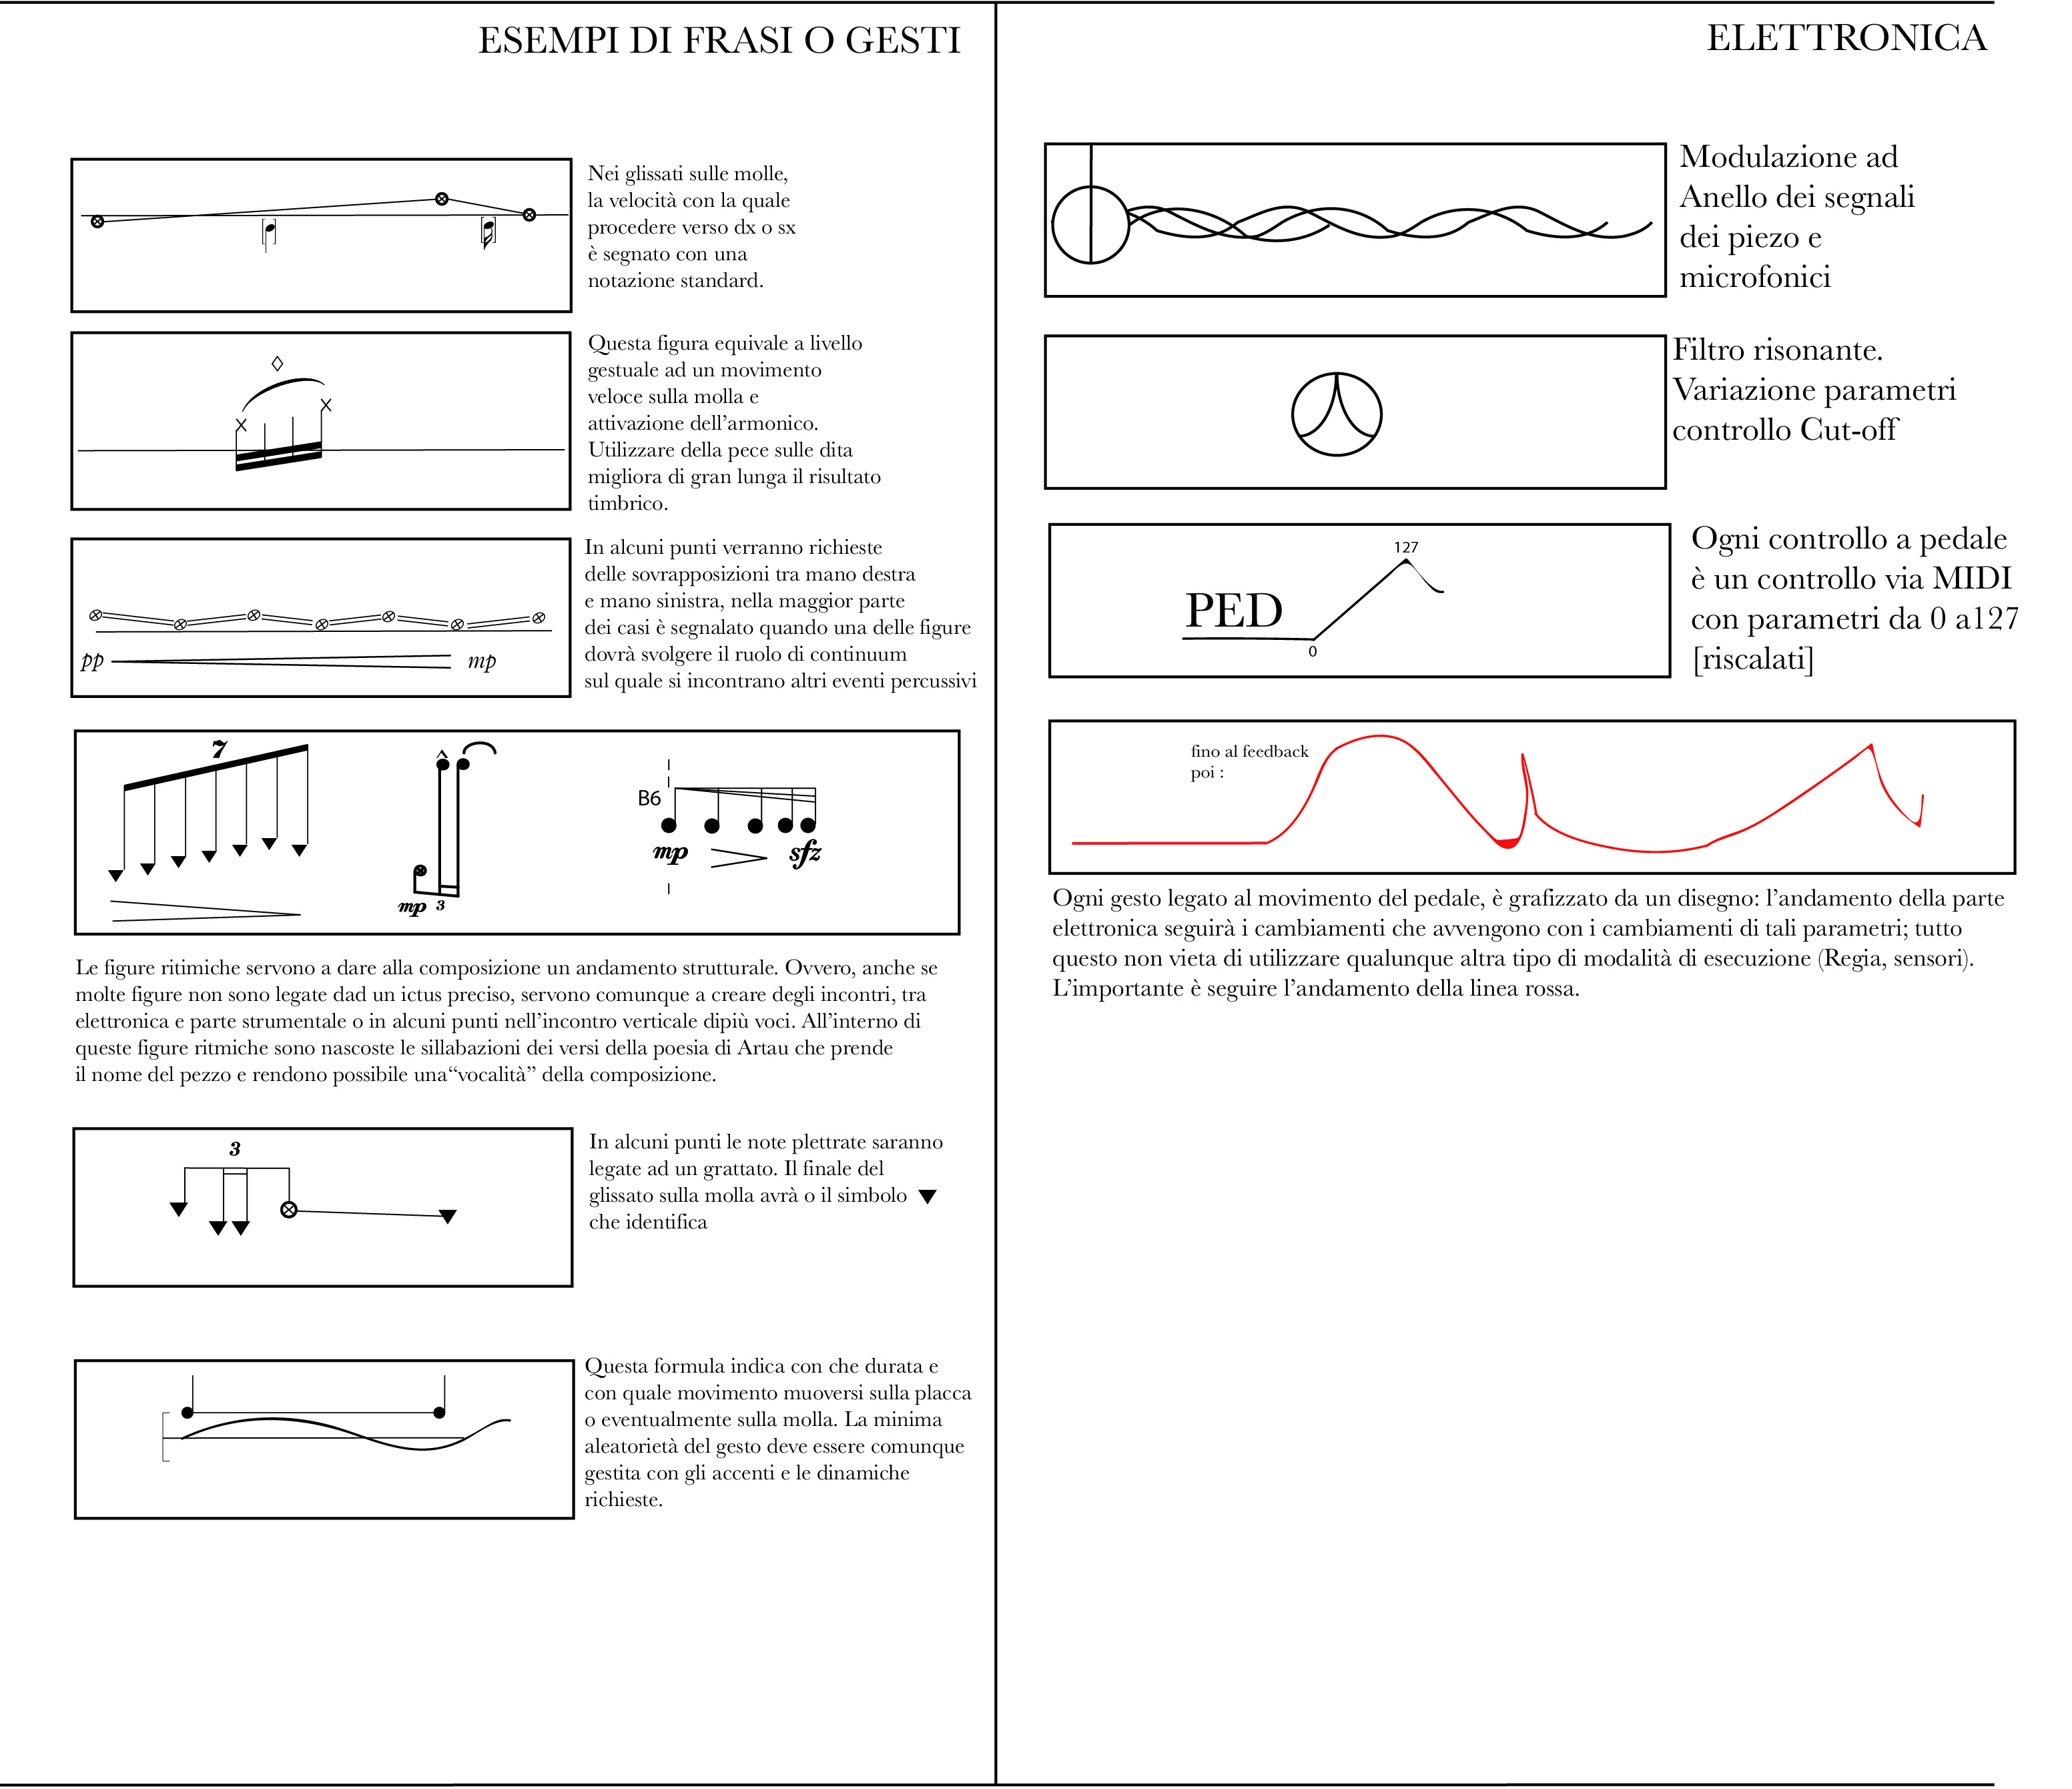
\includegraphics[width=0.6\textwidth]{legenda2.jpg}
\end{minipage}
\end{center}


\section{Algoritmi}
\addcontentsline{toc}{section}{Algoritmi}
\begin{center}
\begin{minipage}[c]{1.\textwidth}
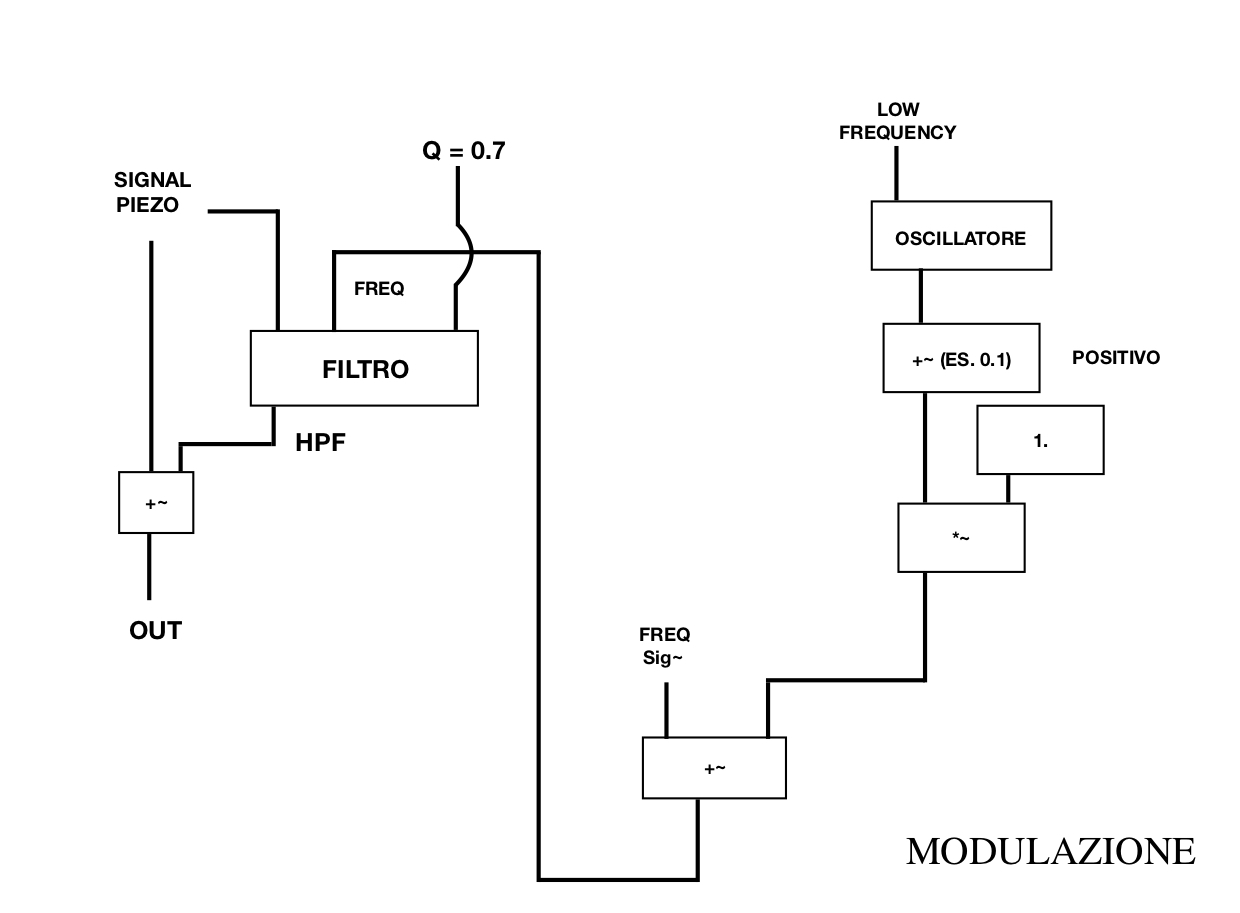
\includegraphics[width=1.\textwidth]{algo_1.jpg}
\end{minipage}
\end{center}
\begin{center}
\begin{minipage}[c]{1.\textwidth}
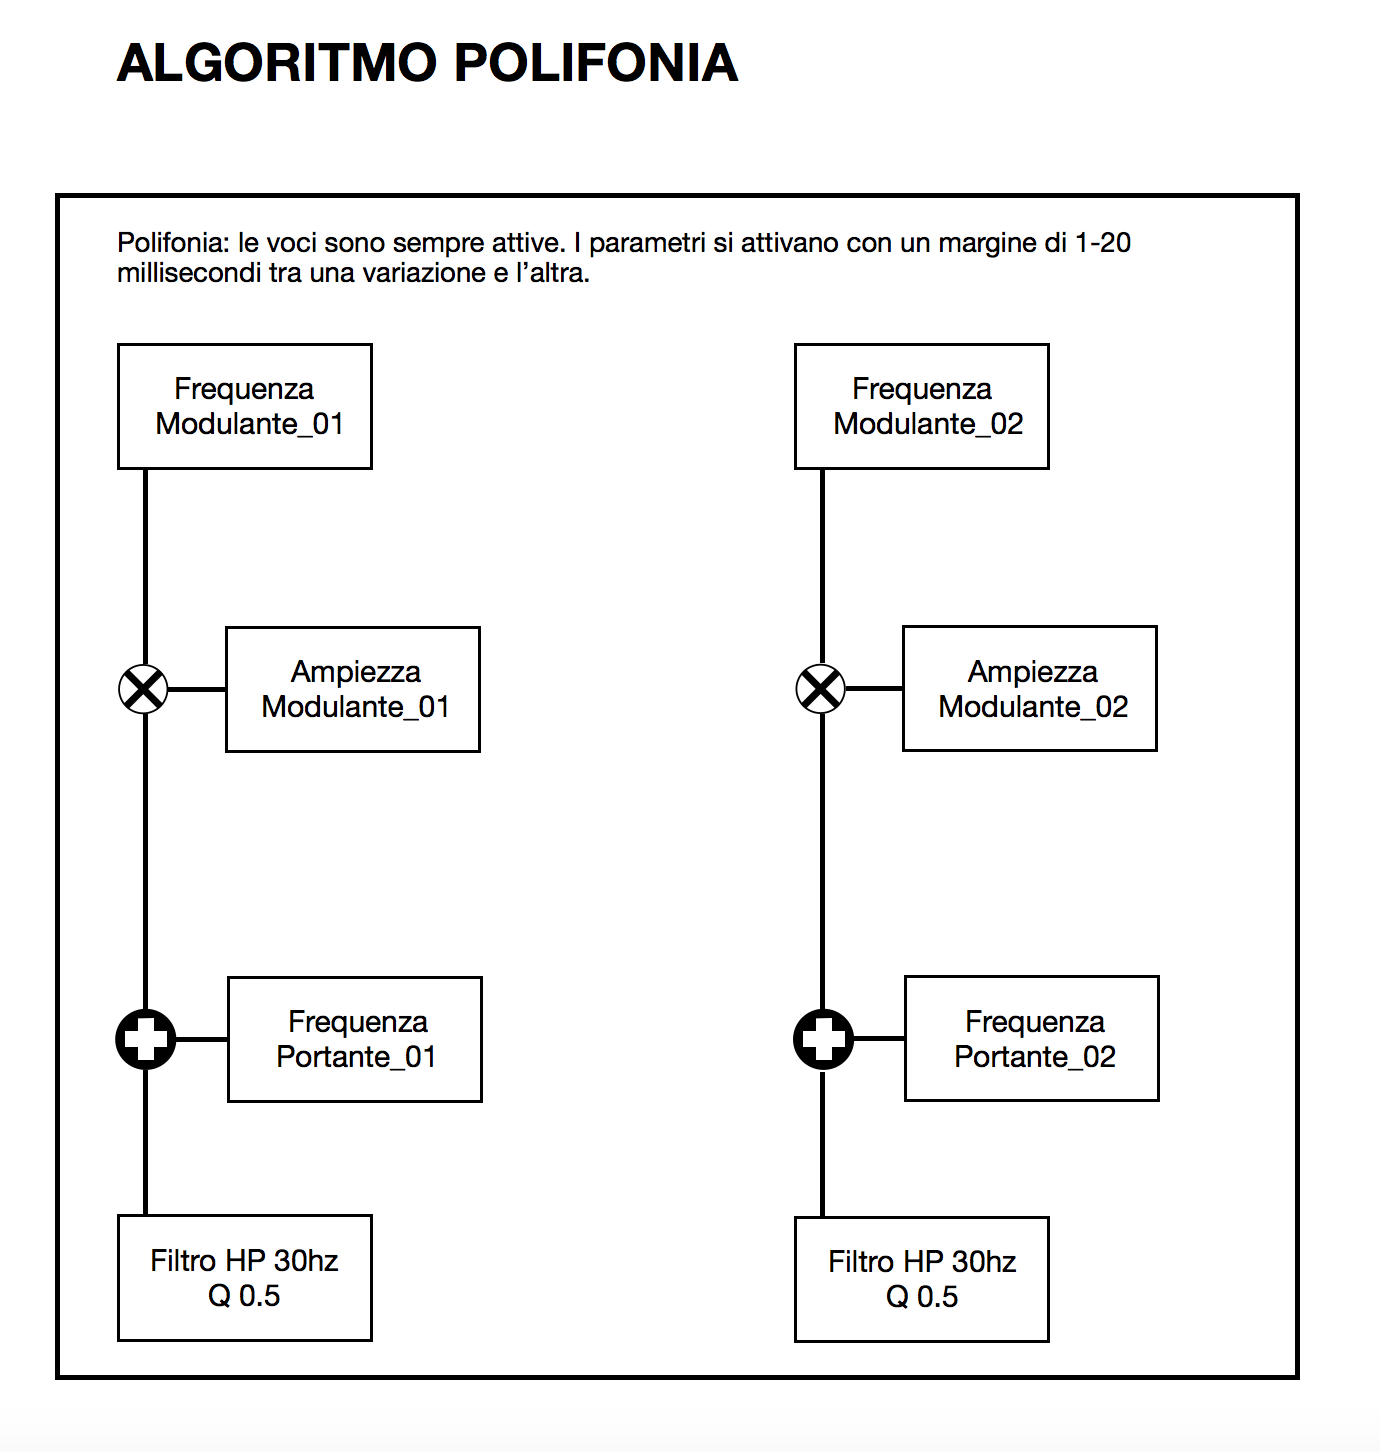
\includegraphics[width=1.\textwidth]{algo_2.jpg}
\end{minipage}
\end{center}


\section{Pedaliera}
\addcontentsline{toc}{section}{Pedaliera}

Pedaliera. Dopo aver studiato il funzionamento ho notato che ogni pulsante numerato era assegnato ad un NOTE on, come una normalissima pedaliera midi per organo. La fortuna � che ogni pulsante equivale a note inerenti al numero presente sulla pedaliera (es. note-on 1 = tasto 1 pedaliera). Quindi essendo identiche, ho solo dovuto trasformare ogni note-on in un ?lancio-scena? sul mio software di utilizzo (max-msp). Questo mi ha facilitato lo studio con il performer che pu� riprovare ogni scena senza dover ripetere temporalmente la sequenza in partitura, ovvero pu� passare ad esempio dalla scena 1 alla scena 6 senza dover ripercorrere tutte le scene presenti tra quelle menzionate. Questo facilita la prova per ogni singolo rigo.


% !TEX TS-program = pdflatex
% !TEX root = ../ArsClassica.tex

%************************************************
\chapter{La ricerca dei materiali (elettromeccanici)}
\label{chp:La ricerca dei materiali (elettromeccanici)}
%************************************************

\begin{tabular}{cp{1cm}p{1cm}p{1cm}} \textbf{Tipologia}&\textbf{Quantit�}&\textbf{Utilizzo}&\textbf{Risposta}\\ 
\hline \textbf{METALLI}\\
\hline Placche metallo&8&Risonatori&Ottima\\
\hline Molle a trazione Inox&2&Strumento&Sufficiente\\
\hline Molle a trazione Acciaio armonico&6&Strumento&Ottima\\
\hline Tubo Quadrato Ferro&2&Basamento&Ottima\\
\hline Viti per innesti&Varie&Bas. Attuatori&Ottima\\
\hline \textbf{VISATON - ATTUATORI}\\
\hline BSX 130 WP - 4 Ohm&4&Vibrazione Placca&Ottima\\ 
\hline ESX 45 - 8 Ohm&4&Vibrazione Placca&Sufficiente\\
\hline ESX 60 - 8 Ohm&3&Vibrazione Placca&Buona\\
\hline \textbf{MAGNETI}\\
\hline Humbucker&2&Amplificazione Molle&Buona\\
\hline Double Coil Bass&1&Amplificazione Molle&Ottima\\
\hline \textbf{PIEZOELETTRICI}\\
\hline Piezoelettrici&4&Amplificazione Molle&Buona\\
\hline 
\end{tabular}

\section{Progettazione e supporto di tiraggio}
\addcontentsline{toc}{section}{Progettazione e supporto di tiraggio}

Le molle a trazione possono arrivare ad una forza di tiraggio pari anche a 100 chili. Per questo l'utilizzo di un basamento adeguato, creato su misura da un fabbro, � la soluzione a qualunque problema relativo al paragrafo 3.3, il fissaggio di attuatori e molle.\\
Il basamento � stato creato grazie all'aiuto di un assistente del Centro di Ricerche Musicali, Leonardo Mammozzetti, che ha visionato e modificato assieme all'autore il progetto del basamento.

\begin{center}
\begin{minipage}[c]{1.\textwidth}
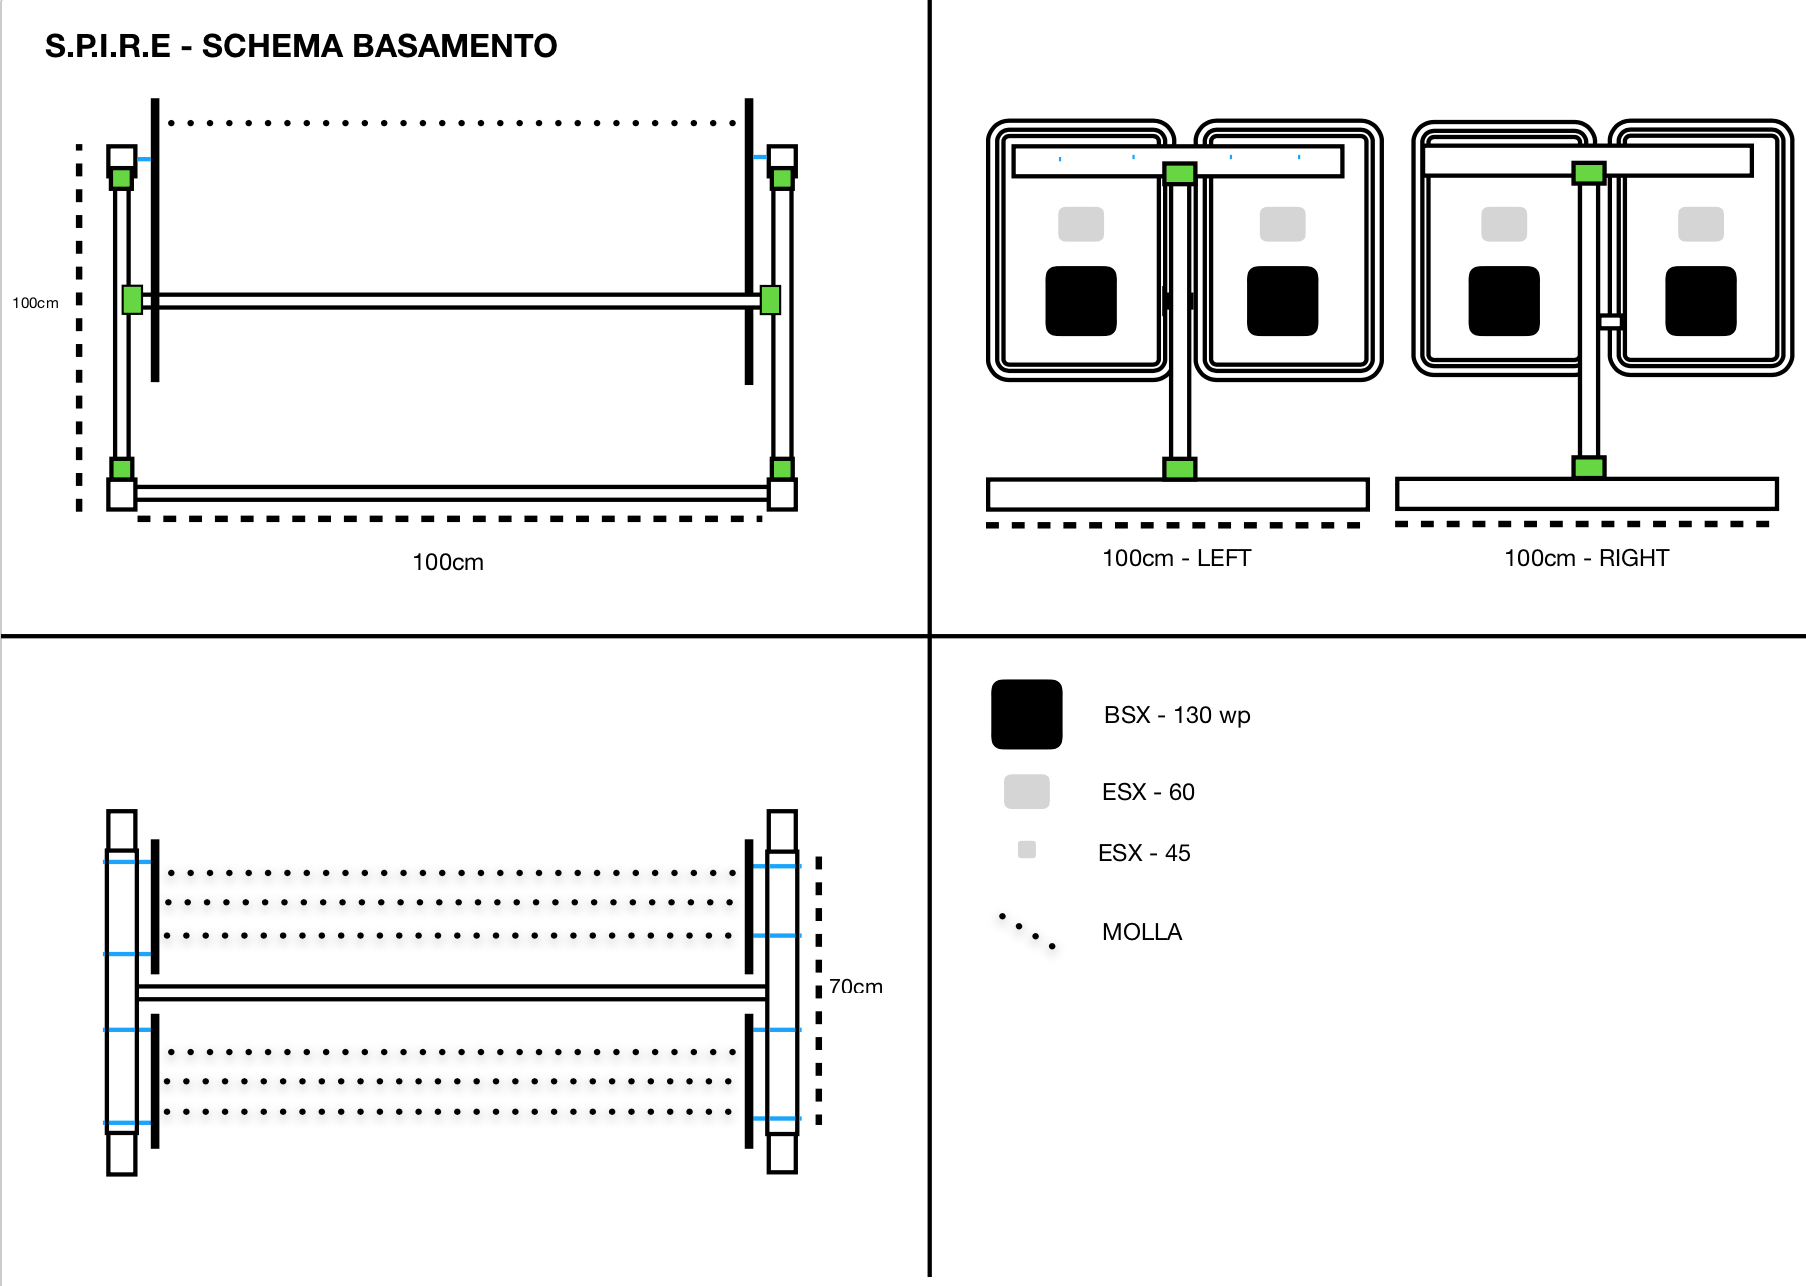
\includegraphics[width=1.\textwidth]{Basamento.jpg}
\end{minipage}
\end{center}

Supporto in ferro. Punti di saldatura in verde. In basso a destra la nomenclatura degli attuatori utilizzati.
In primo luogo la ricerca delle molle. Appena conscio della forma e della natura dello strumento, ho iniziato delle ricerche sulle molle e su le placche (?) in acciaio e ferro armonico. Ho poi contattato il Mollificio Ciullo, ad Albano laziale (Roma) per riuscire ad avere le giuste risposte sulla tipologia delle molle e sul loro funzionamento. Esistono due tipi di molle, del tutto opposte nel loro funzionamento. La natura della molla, a seconda della sua creazione pu� darle delle specifiche del tutto diverso. Le molle prese in esame sono state a (trazione) e a (compressione). 
spiegazione molle a compressione che mi ha portato a visitare un mollificio ad Albano Laziale, il Mollificio Ciullo (\textit{https://www.mollificiociullo.com}) che mi ha esposto le differenze tra le tipologie di molle in commercio e delle peculiarit� elastiche a seconda dei materiali utilizzati. \\
L'acciaio armonico � risultato il materiale migliore per il mio utilizzo perch� a diametri bassi di filatura si possono avere grandi o piccoli diametri per le spire e il risultato non cambia. Ogni molla, se ha un diametro compreso tra 0.1 e 0.2 cm, si ottiene una grande manovrabilit� a livello di flessione e tensione. Da sottolineare che vanno utilizzate solo ed esclusivamente le \underline {Molle a Trazione}; perch� in estensione hanno rigidit� minime anche per lunghezze pari al doppio della loro lunghezza a riposo.
\\
\begin{center}
\begin{minipage}[c]{.7\textwidth}
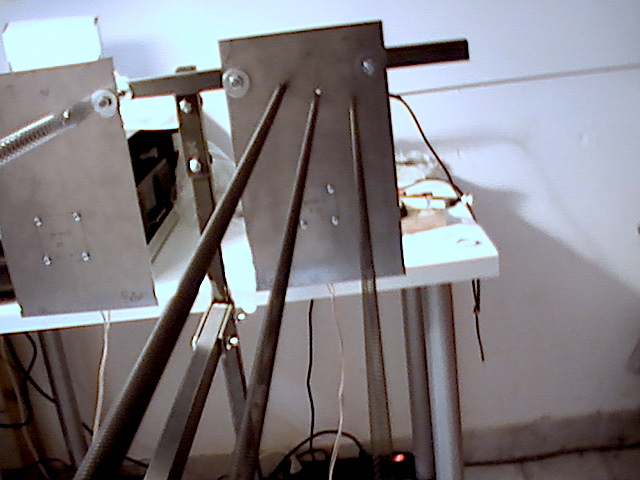
\includegraphics[width=1.\textwidth]{Prototipo2.jpg}
\end{minipage}
\end{center}
Le molle a trazione sono state fissate come in figura, facendo dei buchi sulla lamiera e tese, tutto nella stessa lunghezza, per rendere possibile uno studio omogeneo su materiali diversi che rispondono diversamente al tocco e all'eccitazione mediante attuatori.\\
Si � notato che ogni molla si comporta differentemente a seconda del diametro delle spire, della robustezza del materiale e, ovviamente, del diametro del cavo in acciaio armonico.

\section{Fissaggio Molle e attuatori}
\addcontentsline{toc}{section}{Fissaggio Molle e attuatori}

Gli attuatori sono stati fissati preventivamente tramite del nastro su una delle piastre di metallo e fatte delle prove di risposta del materiale risuonante. Trovato eccellente la risposta del metallo, in questo caso ferro e ferro zigrinato, sono stati segnati dei punti di ancoraggio degli attuatori, tramite viti con rondelle e bulloni. \\ \\
\\
\begin{tabular}{cp{2cm}p{2cm}p{2cm}} \textbf{Tipologia}&\textbf{ATTACCO}&\textbf{BATTENTE}&\textbf{Risposta}\\ 
\hline \textbf{METALLI}\\
\hline Placche metallo&8&Risonatori&Ottima\\
\hline Molle a trazione Inox&2&Strumento&Sufficiente\\
\hline Molle a trazione Acciaio armonico&6&Strumento&Ottima\\
\hline Tubo Quadrato Ferro&2&Basamento&Ottima\\
\hline Viti per innesti&Varie&Bas. Attuatori&Ottima\\
\hline \textbf{MOLLE}\\
\hline BSX 130 WP - 4 Ohm&4&Vibrazione Placca&Ottima\\ 
\hline ESX 45 - 8 Ohm&4&Vibrazione Placca&Sufficiente\\
\hline ESX 60 - 8 Ohm&3&Vibrazione Placca&Buona\\
\hline \textbf{MAGNETI}\\
\hline Humbucker&2&Amplificazione Molle&Buona\\
\hline Double Coil Bass&1&Amplificazione Molle&Ottima\\
\hline \textbf{PIEZOELETTRICI} \\
\hline Piezoelettrici&4&Amplificazione Molle&Buona\\
\hline 
\end{tabular}

\section{Analisi spettrale}
\addcontentsline{toc}{section}{Analisi spettrale}
Di seguito, l'analisi spettrale e lo spettrogramma della risposta all'eccitazione di ogni singola molla. Sottolineo che l'eccitazione della molla, avviene nella parte centrale. \\
\begin{center}
\begin{minipage}[c]{1.\textwidth}
\includegraphics[width=1.\textwidth]{MOLLA1.jpg}
\end{minipage}
\end{center}
\begin{center}
\begin{minipage}[c]{1.\textwidth}
\includegraphics[width=1.\textwidth]{MOLLA2.jpg}
\end{minipage}
\end{center}
\begin{center}
\begin{minipage}[c]{1.\textwidth}
\includegraphics[width=1.\textwidth]{MOLLA3.jpg}
\end{minipage}
\end{center}
\begin{center}
\begin{minipage}[c]{1.\textwidth}
\includegraphics[width=1.\textwidth]{MOLLA4.jpg}
\end{minipage}
\end{center}

Ogni molla � soggetta ad un inviluppo e un decadimento differente, questo porta, a livello compositivo, a gestire sia timbri che dinamiche diverse per lavorare sia sulla parte orizzontale della stesura compositiva che verticale. Gli incastri formali consisteranno, infatti in \textit{crescendo} dinamici legati soprattutto ai rapporti timbrici tra le molle.


\section{Schema Elettrico}
\addcontentsline{toc}{section}{Schema Elettrico}
Di seguito, lo schema elettrico per il collegamento degli attuatori:
\begin{center}
\includegraphics[width=1.\textwidth]{Elettrico.jpg}
\end{center}



% !TEX TS-program = pdflatex
% !TEX root = ../ArsClassica.tex

%************************************************
\chapter{Sistema di diffusione)}
\label{chp:Sistema di diffusione}
%************************************************

\epigraph{Come un rosone nel cuore di un tempio immenso}{\textit{Antonin Artaud}}

\section{Sistema di ripresa}
\addcontentsline{toc}{section}{Sistema di ripresa}
La diffusione audio avverr� tramite l'utilizzo di un sistema di diffusione omnidirezionale che render� possibile la diffusione omogenea del materiale acustico ed elettronico prodotto da Sp.i.r.e.. \\
Strumenti utilizzati:
\begin{center}
\begin{minipage}[c]{1.\textwidth}
\includegraphics[width=1.\textwidth]{Diffusione.jpg}
\end{minipage}
\end{center}
\begin{itemize}
	\item{Sp.i.r.e.}
\end{itemize}

Tutti gli studi sono stati fatti su acciaio armonico o acciaio inox. Due sono i fattori che regolano il funzionamento della molla a trazione:
\begin{enumerate}
\item{Diametro del filo}
\item{Larghezza del diametro esterno (\textit{spira})}
\end{enumerate}
Il diametro del filo (1.) unito alla larghezza del diametro esterno (2.) rendono possibile il cambiamento della qualit� della flessione della molla. Anche il numero di spire agisce sulla flessione della molla.

\section{Diffusione audio e B-Format}
\addcontentsline{toc}{section}{Diffusione audio e B-Format}

Per la costruzione del sistema di diffusione ho utilizzo gli scritti introduttivi che sono allegati a molte partiture di Luigi Nono (cit. postpraeludium e Prometeo). Ovvero, il compositore non � pi� slegato da una realt� percettiva e teatrale del produzione sonora, ma diventa artefice della disposizione degli altoparlanti, del pubblico e della quantit� di persone che possono simultaneamente partecipare all'esecuzione del pezzo. \\
Vitres de son ha un ascolto ottimale in una configurazione sonor

Sistema di diffusione:
\begin{itemize}
	\item{Scheda Audio 8in 8out}
	\item{Cablaggio}
	\item{2 Amplificatori di potenza da 4 canali a 4 Ohm}
	\item{Computer}
\end{itemize}




% !TEX TS-program = pdflatex
% !TEX root = ../ArsClassica.tex

%************************************************
\chapter{Riflessioni e conclusioni}
\label{chp:Riflessioni e conclusioni}
%************************************************

La strada percorsa fino a questo momento non delinea la fine di un percorso, ma bens� uno step. Un varco importante verso una determinata considerazione degli eventi musicali e dell'evoluzioni del suono.
La strada percorsa fino ad ora non arriva a delineare la fine di un percorso, ma piuttosto un inizio. \\
Questo lavoro di tesi lo identifico di pi� come un percorso costruito su un ponte che ancora sto attraversando che mi spinge sempre pi� verso una consapevolezza artistica. Tale consapevolezza rende giorno per giorno meno vacillanti le fondamenta di questo ponte di transito verso una maturit� stilistica: � la drammaturgia di una struttura musicale in divenire. \\
L'idea che ogni frase, sia ritmica che melodica, risulto come un entit� a s� � il passo odierno e sul quale voglio continuare le mie ricerche formali. Ogni modifica, ogni variazione, � legata ad un determinato personaggio musicale, che si modifica nell'aspetto e nella forma durante ogni cambiamento di oggetti/esseri limitrofi. \\
Anche a livello compositivo cercher� di esprimere tale costrutto: l'identit� di ogni struttura dovr� essere ben salda ed ogni suo mutamento risultare pieno di un proprio significato espressivo, colmo di quella trasformazione intrinseca alle modifiche sul materiale sonoro. Vorrei che il mio studio compositivo futuro sia un lungo viaggio: verso la conoscenza di altre identit� in trasformazione che incontrer� lungo le strade e i percorsi che purtroppo o per fortuna la vita ci propina, sempre con la speranza di una nascita nella quale si veda il sole.



\clearpage

% !TEX TS-program = pdflatex
% !TEX root = ../ArsClassica.tex

%*******************************************************
% Bibliography
%*******************************************************
\nocite{*}
\printbibliography

\end{document}
